\documentclass[10pt, conference]{IEEEtran/IEEEtran}

\usepackage{graphicx}
\usepackage{color}
\usepackage{amsmath}
\usepackage{float}
\usepackage[all]{xy}
\usepackage[font=small]{caption}
\usepackage{hyperref}


\begin{document}

\title{Performance Analysis of TCP Variants}

\author{\IEEEauthorblockN{Liang Tian}
\IEEEauthorblockA{College of Computer and Information Science\\
Northeastern University, MA, 02115\\
Email: ltian@ccs.neu.edu\\}
\and
\IEEEauthorblockN{Yang Cai}
\IEEEauthorblockA{College of Computer and Information Science\\
Northeastern University, MA, 02115\\
Email: yang@ccs.neu.edu\\}
}
\maketitle
\begin{abstract}
In this paper we conducted simulation-based experiments to analyze performance of  TCP variants Tahoe, Reno, 

\end{abstract}
\section{Introduction}
\section{Methodology}

\subsection{Tools}
- NS-2: simulation, which runs the experiment with given configuration, and
  output a trace file that we can analyze packets transmission.
- tcl: conduct simulation,
- and Python, analyze trace and plot graphs




\subsection{Notations}

We define throughput, latency, drop-rate as follows:

\[
\text{throughput}= \frac{\text{\# of received packets} \cdot \text{packet size}}{duration}
\]
where we count the number of received ACKs at the sender agent 
\[
\text{latency}=\frac{\text{sum of RTT of all received packets} }{\text{\# of packets received}}
\]
\[
\text{drop-rate}: \frac{\text{(\# sent packets - \# received packets)}}{\text{\# sent packets}}
\]
\section{Experiments}
In all experiments below, we use the same simple network topology as shown in the following graph:

\centerline{
\xymatrix{
N1 \ar@{-}[dr] & & & N4\\
& N2\ar@{-}[r]  & N3\ar@{-}[dr] \ar@{-}[ur]  & \\
N5\ar@{-}[ur]  &  &  & N6\\
}
}

\subsection{Experiment 1: TCP Performance Under Congestion}
\subsubsection{Configuration}

CBR source at N2 and sink at N3, one single TCP stream from N1 to N4.

Do experiments for each combination of the following, each runs 10 times:
- CBR from 1 to 10 Mbps 
- TCP variants Tahoe, Reno, NewReno and Vegas.
- different delay of each link
- different random seed
- different packet size

For each setup, run the experiment 100 times and take the average
after computing throughput, latency and drop-rate by using Python to analyze the
trace of NS2. Observe the different behavior of each protocol under same
circumstances, and whether the packet size/delay/random seed would
influence their behaviors. If delay of each link has obvious effect on the result,
fast re-transmission may be the reason. If average result of two protocol is different by more than
10\% under different situations, then it would be statistically significant result.
\subsubsection{Results Analysis}

\begin{figure}[htbp]
\begin{center}
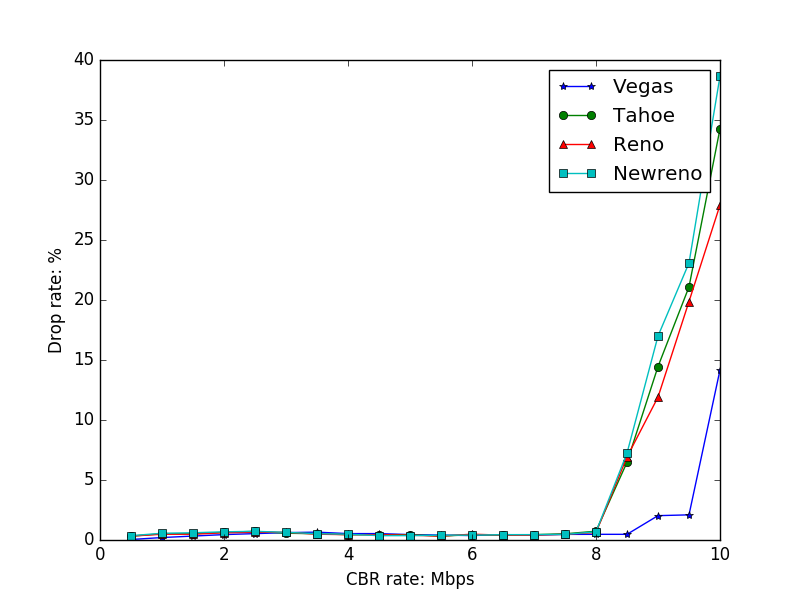
\includegraphics[width=\linewidth]{../exp1/exp1_drop.png}
\caption{Drop rate of TCP variants under different CBR rates}
\label{exp1_drop}
\end{center}
\end{figure}

\begin{figure}[htbp]
\begin{center}
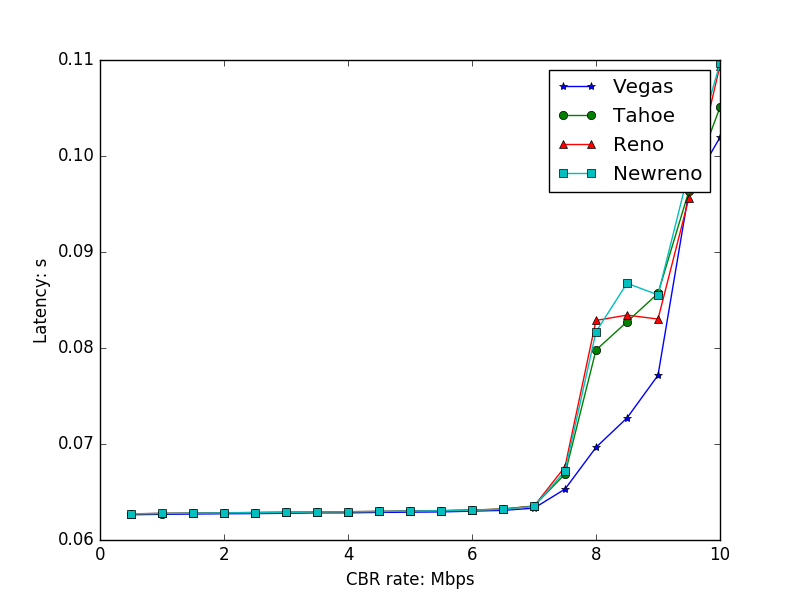
\includegraphics[width=\linewidth]{../exp1/exp1_lat.png}
\caption{Latency of TCP variants under different CBR rates}
\label{exp1_lat}
\end{center}
\end{figure}

\begin{figure}[htbp]
\begin{center}
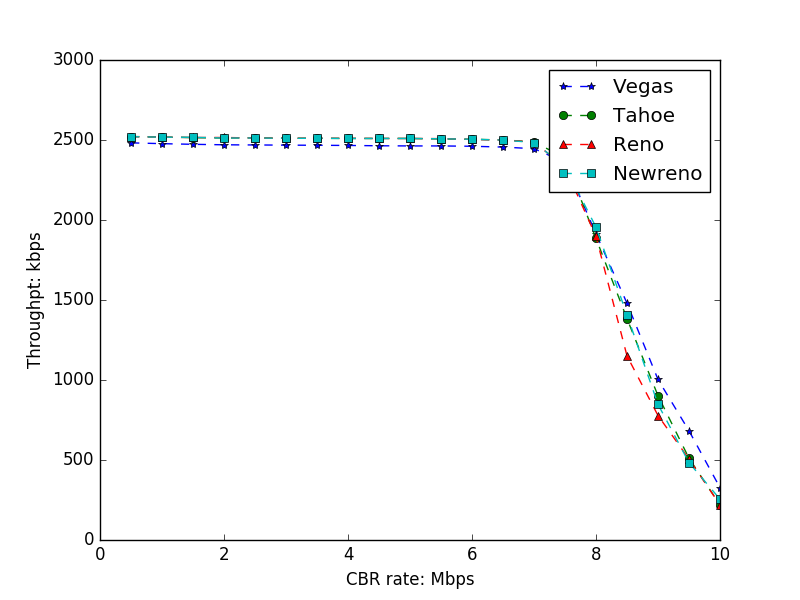
\includegraphics[width=\linewidth]{../exp1/exp1_thpt.png}
\caption{Throughput of TCP variants under different CBR rates}
\label{exp1_thpt}
\end{center}
\end{figure}




\subsection{Experiment 2: Fairness Between TCP Variants}


CBR source at N2 and sink at N3, one TCP stream from N1 to N4 using one TCP
variant and another TCP stream from N5 to N6 using another TCP variant.

Do experiments for each combination of the following, each runs 10 times:
- Each pair of TCP variants(one of Reno/Reno, NewReno/Reno, Vegas/Vegas,
NewReno/Vegas), 
- CBR from 1 to 10Mbps.
- different start time
- different random seed

Compute throughput, latency and drop-rate by using Python to analyze the
trace of NS2 and plot average for runs of the same configuration. If the results
vary under different start time, it should be that AIMD algorithm is effecting on fairness.
If the difference between two protocol is more than 10\% under different situations, then it would be
the statistically significant result.

%Reno/Reno
\subsubsection{Reno/Reno}
\begin{figure}
\begin{center}
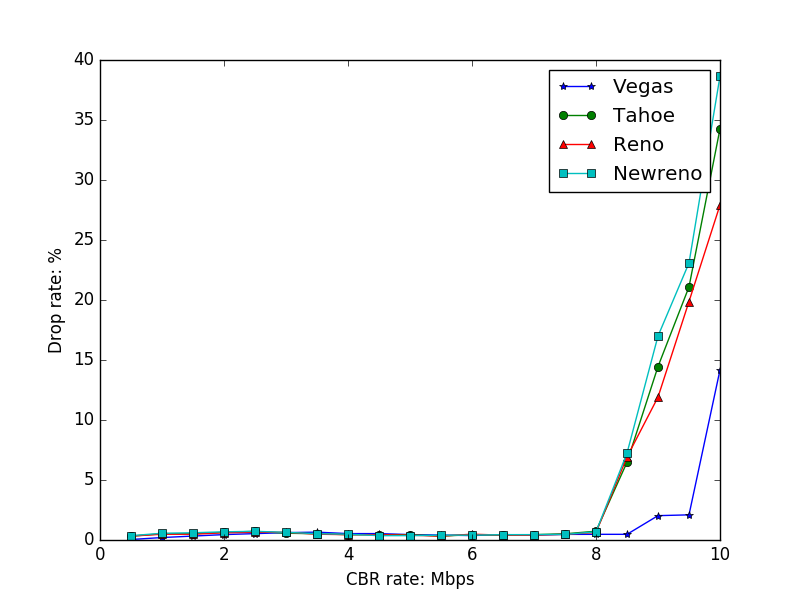
\includegraphics[width=\linewidth]{../exp1/exp1_drop.png}
\caption{Drop rate of TCP variants under different CBR rates}
\label{exp1_drop}
\end{center}
\end{figure}

\begin{figure}[htbp]
\begin{center}
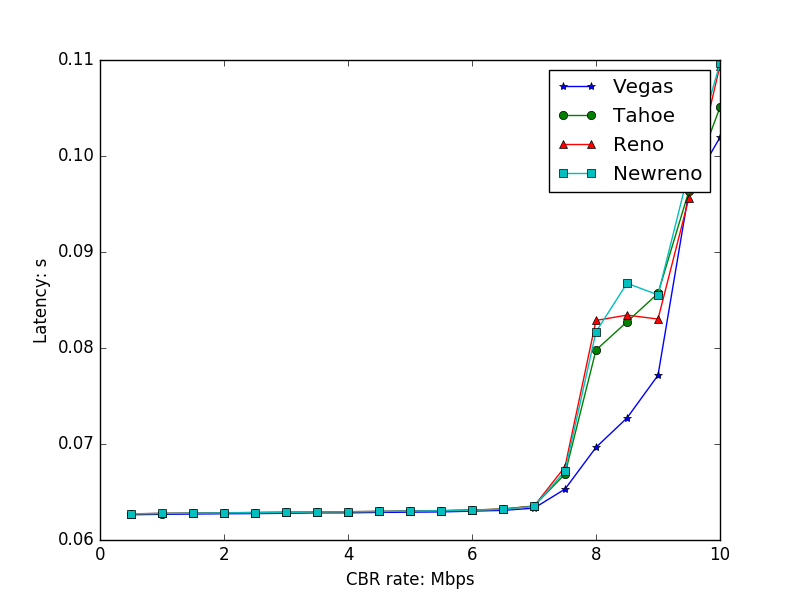
\includegraphics[width=\linewidth]{../exp1/exp1_lat.png}
\caption{Latency of TCP variants under different CBR rates}
\label{exp1_lat}
\end{center}
\end{figure}

\begin{figure}[htbp]
\begin{center}
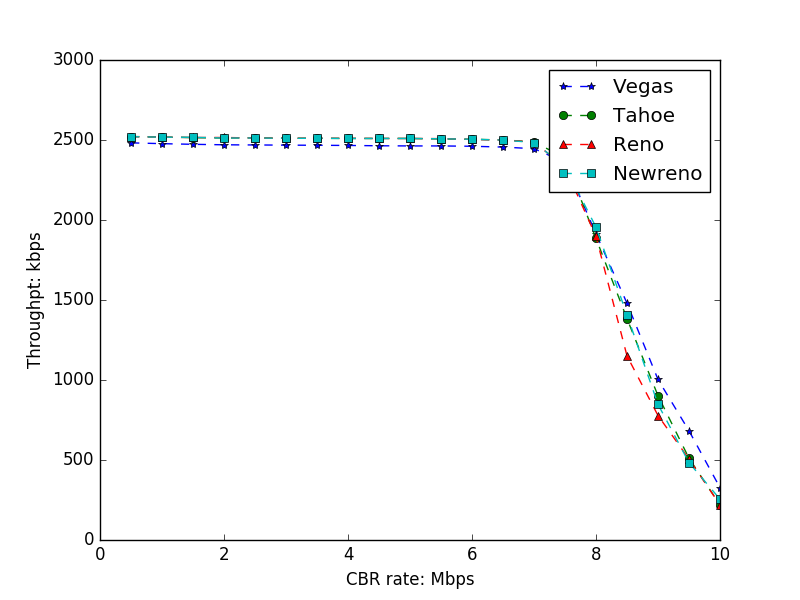
\includegraphics[width=\linewidth]{../exp1/exp1_thpt.png}
\caption{Throughput of TCP variants under different CBR rates}
\label{exp1_thpt}
\end{center}
\end{figure}

%NewReno/Reno
\subsubsection{NewReno/Reno}
By comparing the drop-rate , throughput and latency of the two TCP streams,  we can see that their performances are very similar, so Reno is fair to itself. 
%Why?

\begin{figure}[htbp]
\begin{center}
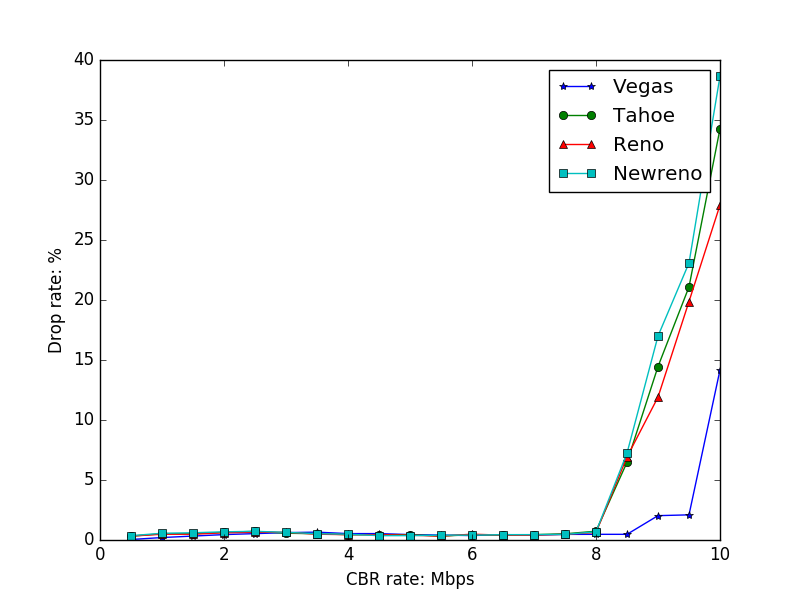
\includegraphics[width=\linewidth]{../exp1/exp1_drop.png}
\caption{Drop rate of TCP variants under different CBR rates}
\label{exp1_drop}
\end{center}
\end{figure}

\begin{figure}[htbp]
\begin{center}
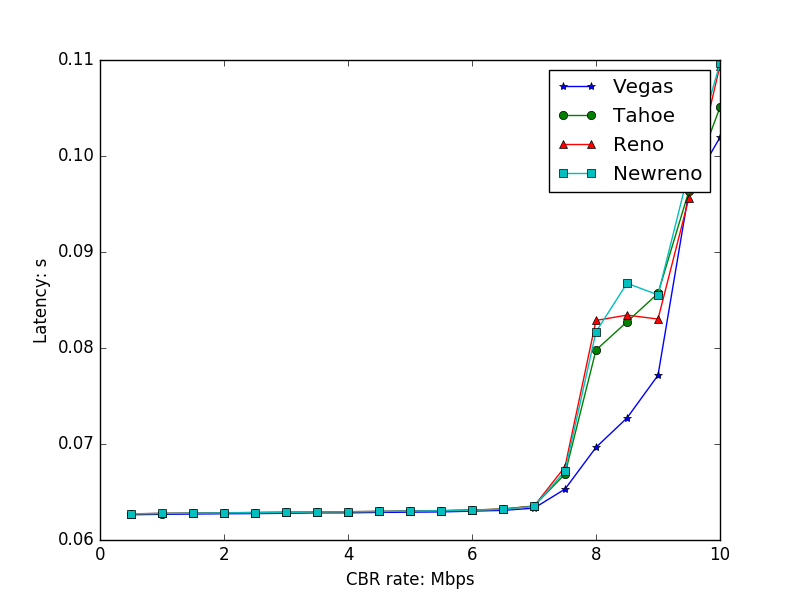
\includegraphics[width=\linewidth]{../exp1/exp1_lat.png}
\caption{Latency of TCP variants under different CBR rates}
\label{exp1_lat}
\end{center}
\end{figure}

\begin{figure}[htbp]
\begin{center}
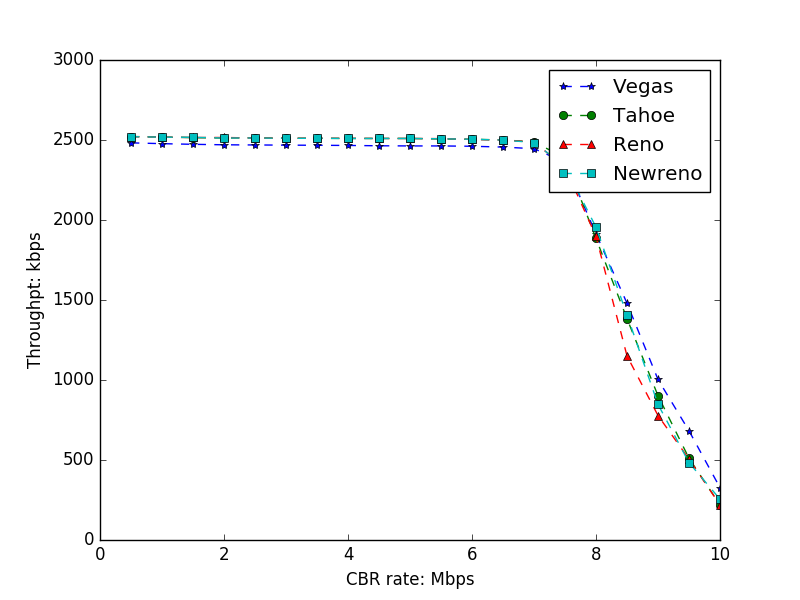
\includegraphics[width=\linewidth]{../exp1/exp1_thpt.png}
\caption{Throughput of TCP variants under different CBR rates}
\label{exp1_thpt}
\end{center}
\end{figure}

\subsubsection{Vegas/Vegas}
% only 1 figure here.
This case is similar to what we saw with Reno/Reno, Vegas is fair to itself, as shown below. Another interesting observation is that % I guess latency would be 
\begin{figure}[htbp]
\begin{center}
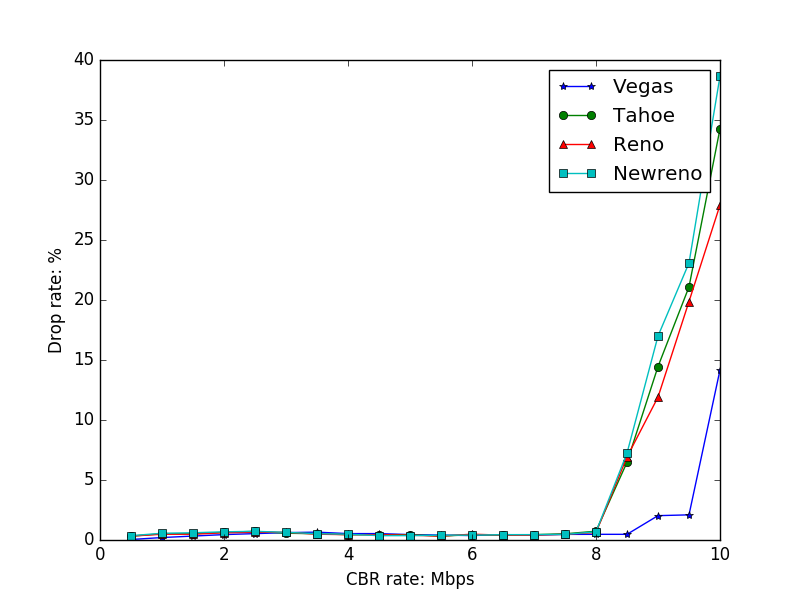
\includegraphics[width=\linewidth]{../exp1/exp1_drop.png}
\caption{Drop rate of TCP variants under different CBR rates}
\label{exp1_drop}
\end{center}
\end{figure}

%NewReno/Vegas
\subsubsection{NewReno/Vegas}

%TCP Vegas is a TCP congestion avoidance algorithm that emphasizes packet delay, rather than packet loss, as a signal to help determine the rate at which to send packets. It was developed at the University of Arizona by Lawrence Brakmo and Larry L. Peterson.[1][2]
%
%TCP Vegas detects congestion at an incipient stage based on increasing Round-Trip Time (RTT) values of the packets in the connection unlike other flavors such as Reno, New Reno, etc., which detect congestion only after it has actually happened via packet loss. The algorithm depends heavily on accurate calculation of the Base RTT value. If it is too small then throughput of the connection will be less than the bandwidth available while if the value is too large then it will overrun the connection.
%
%A lot of research is going on regarding the fairness provided by the linear increase/decrease mechanism for congestion control in Vegas. 
Performance of Vegas degrades because Vegas reduces its sending rate before New Reno, as it detects congestion early and hence gives greater bandwidth to co-existing TCP Reno flows.

TCP Vegas is one of several "flavors" of TCP congestion avoidance algorithms. It is one of a series of efforts at TCP tuning that adapt congestion control and system behaviors to new challenges faced by increases in available bandwidth in Internet components on networks like Internet2.[7][8]

%TCP Vegas has been implemented in the Linux kernel,[9] in FreeBSD[10] and possibly in other operating systems as well.

\begin{figure}[htbp]
\begin{center}
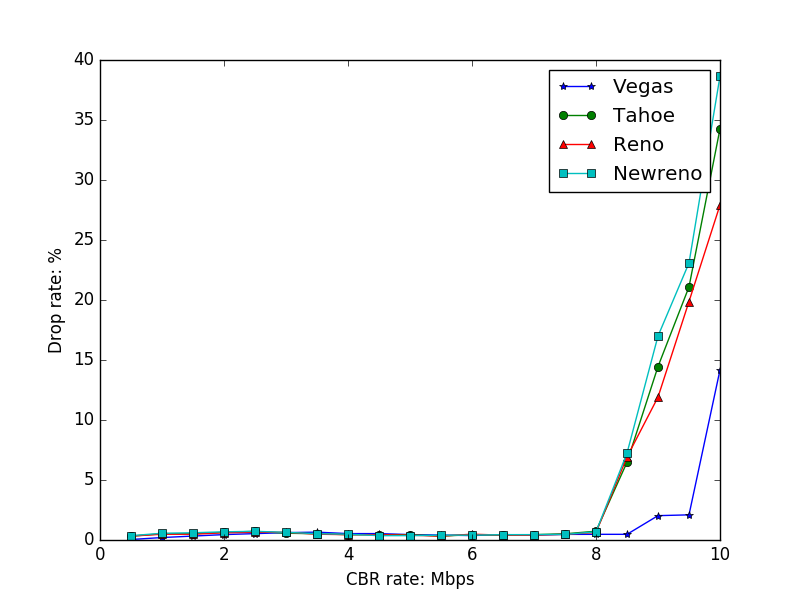
\includegraphics[width=\linewidth]{../exp1/exp1_drop.png}
\caption{Drop rate of TCP variants under different CBR rates}
\label{exp1_drop}
\end{center}
\end{figure}

\begin{figure}[htbp]
\begin{center}
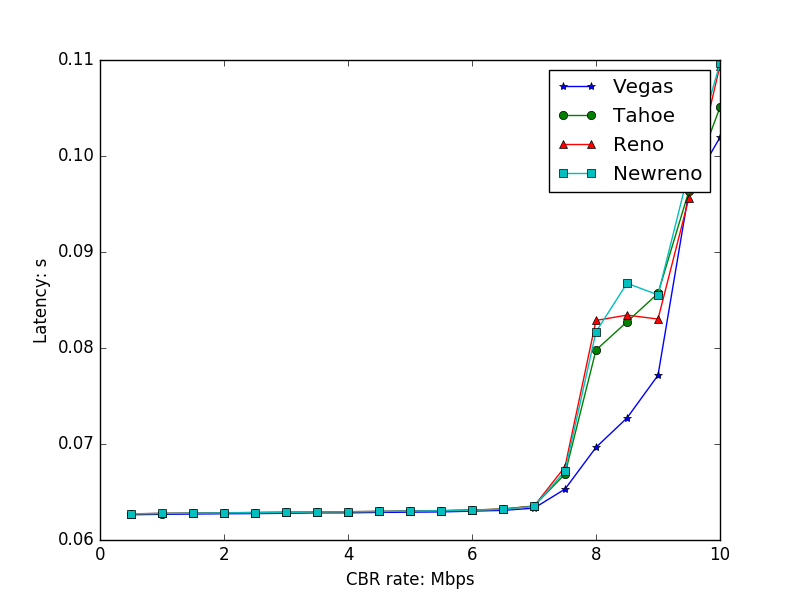
\includegraphics[width=\linewidth]{../exp1/exp1_lat.png}
\caption{Latency of TCP variants under different CBR rates}
\label{exp1_lat}
\end{center}
\end{figure}

\begin{figure}[htbp]
\begin{center}
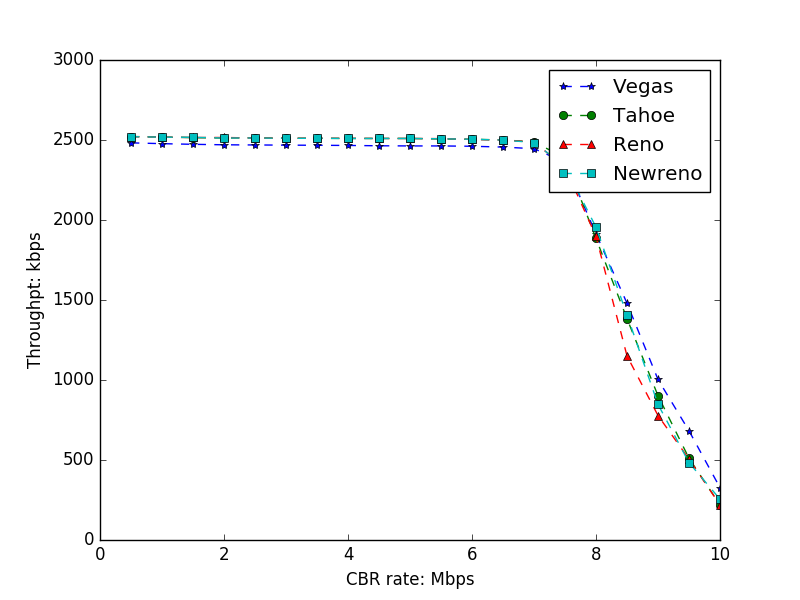
\includegraphics[width=\linewidth]{../exp1/exp1_thpt.png}
\caption{Throughput of TCP variants under different CBR rates}
\label{exp1_thpt}
\end{center}
\end{figure}




\subsection{Experiment 3: Influence of Queuing}

\subsubsection{Configuration}

For each queueing algorithm DropTail and RED:

Use TCP Reno and SACK to create two TCP flows N1 to N4 and N5 to N6, after 5 
seconds, introduce CBR from N2 to N3. Repeat the experiment for different CBR 
bandwidths.

\subsubsection{Results Analysis}

\begin{figure}[htbp]
\begin{center}
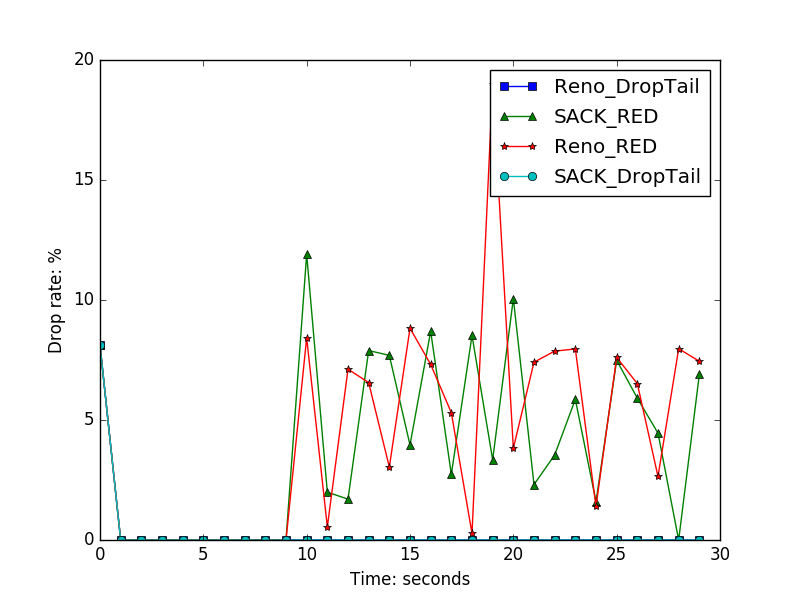
\includegraphics[width=\linewidth]{../exp3/exp3_drop.png}
\caption{Drop rate of TCP variants with different queueing algorithm}
\label{exp1_drop}
\end{center}
\end{figure}

\begin{figure}[htbp]
\begin{center}
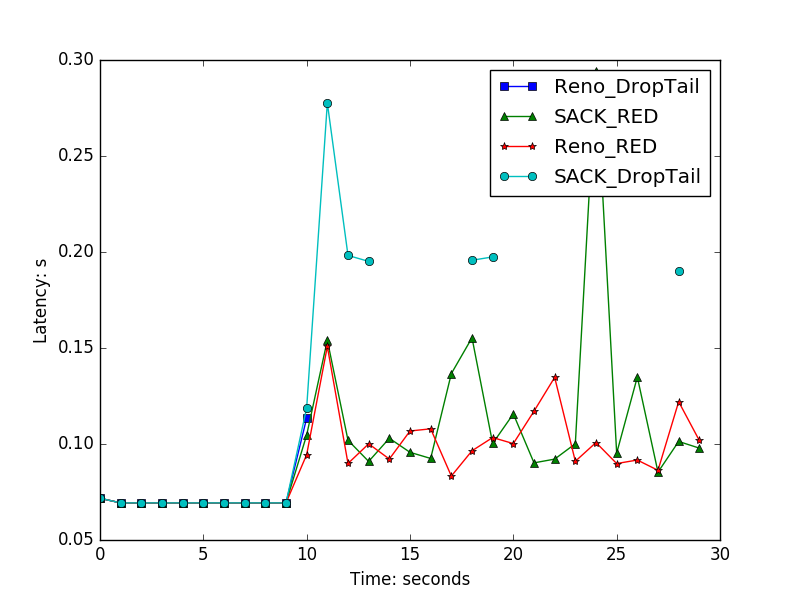
\includegraphics[width=\linewidth]{../exp3/exp3_lat.png}
\caption{Latency of TCP variants with different queueing algorithm}
\label{exp1_lat}
\end{center}
\end{figure}

\begin{figure}[htbp]
\begin{center}
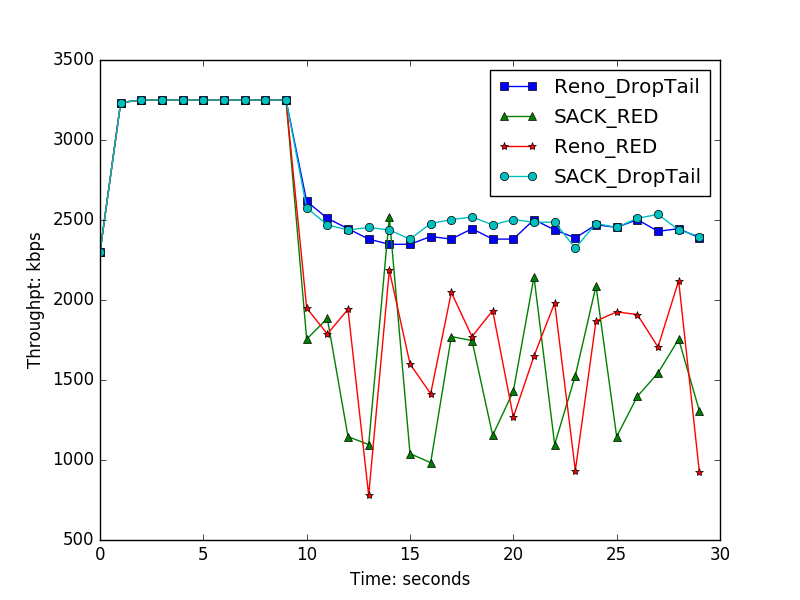
\includegraphics[width=\linewidth]{../exp3/exp3_thpt.png}
\caption{Throughput of TCP variants with different queueing algorithm}
\label{exp1_thpt}
\end{center}
\end{figure}
\section{Conclusion}

\section{References}
\url{https://en.wikipedia.org/wiki/TCP_Vegas}


\end{document}